% SPDX-FileCopyrightText: Copyright © 2026-present Sedimentologika
% SPDX-FileContributor: Jarred C. Lloyd
%
% SPDX-License-Identifier: LPPL-1.3c
% ======================================================================================== %
%       LaTeX pre-print and submission and production template for Sedimentologika         %
%                v1.1.2 - July 2026, Sedimentologika Steering Committee                    %
% ======================================================================================== %
%    This template and corresponding class are provided as is. Sedimentologika takes no
%                  responsibility for your misuse of the provided files.
%
%                       It MUST be compiled using LuaLaTeX.
%             TeXLive 2024 or higher, and Overleaf should work without issue.
%                         Tested on TeXLive 2024, 2025, 2026
%      Note: free accounts on Overleaf may time out during compilation due to the use of
%             unicode-math. We will switch to lua-unicode-math when it in future.
%
%   There are comments throughout this tex file to assist you in generating your document.
%
%      If you are unable to compile your document and are using LuaLaTeX, first consult
%                the README.md file, then if you need further assistance
%                       contact us via support@sedimentologika.org
%
%     If you discover a reproducible bug, please document the steps to reproduce it and
%                      let the team know via support@sedimentologika.org
%
% ======================================================================================== %
%                                    Document class                                        %
% ======================================================================================== %
% INSTRUCTION: change the content in square brackets to suit your needs using the below
% options
% ---------------------------------------------------------------------------------------- %
\documentclass[preprint]{sedimentologika}
% ---------------------------------------------------------------------------------------- %
%
% [preprint] to enable pre-print styling
%
% INSTRUCTION: If generating a pre-print, review the below statement and alter to
% your needs.
\preprintdeclaration{
  This is a pre-print and has not yet undergone peer-review.
  It has been submitted to \textit{Sedimentologika}.
}
%
% [submission] to enable submission styling suitable for Sedimentologika
%
% [submission, anonymous] to enable submission styling suitable for Sedimentologika
%       The 'anonymous' option removes author names and attempts to strip metadata from the %       generated PDF.
%
%       IMPORTANT: It is the authors' responsibility to ensure that no identifying
%       information remains in the file.
%
%       Sedimentologika is NOT RESPONSIBLE for any failure by the authors' to maintain
%       anonymity during file generation or submission.
%       If anonymity is requested, we will uphold it throughout the review process.
%
%       Note: Posting a pre-print is strongly encouraged. However, doing so may compromise
%       anonymity, as the file becomes publicly accessible and searchable online.
%
% ======================================================================================== %
%                                  Document languages                                      %
% ======================================================================================== %
% INSTRUCTION: Change the language in the curly braces to a valid English dialect from the
% babel package (english, american, australian, british, canadian, newzealand) that you
%  will use for your manuscript
% ---------------------------------------------------------------------------------------- %
\englishvariety{australian}
% ---------------------------------------------------------------------------------------- %
%
% ---------------------------------------------------------------------------------------- %
% ADVANCED USAGE FOR NON-ROMAN ALPHABET LANGUAGE SUPPORT IN TRANSLATION
% ---------------------------------------------------------------------------------------- %
% The below commented out code is an example for enabling non-roman alphabet (e.g. Arabic)
% language support. You will need to have the appropriate Noto Sans font installed on your
% system. Contact support@sedimentologika.org if you are unable to get this working.
% This is an advanced usage. On Overleaf, the below commented out code will enable appropriate fonts in Arabic, Japanese, Chinese (simplified), and Korean.
%
% \babelfont[arabic]{rm}[%
%   Path={translation-fonts/},
%   BoldFont={NotoSansArabic-VariableFont_wdth,wght.ttf},
%   Numbers={Proportional,Lining},
%   UprightFeatures={Weight=350},
%   BoldFeatures={Weight=600}
% ]{NotoSansArabic-VariableFont_wdth,wght.ttf}
% \babelfont[arabic]{sf}[%
%   Path={translation-fonts/},
%   BoldFont={NotoSansArabic-VariableFont_wdth,wght.ttf},
%   Numbers={Proportional,Lining},
%   UprightFeatures={Weight=350},
%   BoldFeatures={Weight=600}
% ]{NotoSansArabic-VariableFont_wdth,wght.ttf}
% \babelfont[japanese]{rm}[%
%   Path={translation-fonts/},
%   BoldFont={NotoSansJP-VariableFont_wght.ttf},
%   Numbers={Proportional,Lining},
%   UprightFeatures={Weight=350},
%   BoldFeatures={Weight=600}
% ]{NotoSansJP-VariableFont_wght.ttf}
% \babelfont[japanese]{sf}[%
%   Path={translation-fonts/},
%   BoldFont={NotoSansJP-VariableFont_wght.ttf},
%   Numbers={Proportional,Lining},
%   UprightFeatures={Weight=350},
%   BoldFeatures={Weight=600}
% ]{NotoSansJP-VariableFont_wght.ttf}
% \babelfont[korean]{rm}[%
%   Path={translation-fonts/},
%   BoldFont={NotoSansKR-VariableFont_wght.ttf},
%   Numbers={Proportional,Lining},
%   UprightFeatures={Weight=350},
%   BoldFeatures={Weight=600}
% ]{NotoSansKR-VariableFont_wght.ttf}
% \babelfont[korean]{sf}[%
%   Path={translation-fonts/},
%   BoldFont={NotoSansKR-VariableFont_wght.ttf},
%   Numbers={Proportional,Lining},
%   UprightFeatures={Weight=350},
%   BoldFeatures={Weight=600}
% ]{NotoSansKR-VariableFont_wght.ttf}
% \babelfont[chinese-simplified]{rm}[%
%   Path={translation-fonts/},
%   BoldFont={NotoSansSC-VariableFont_wght.ttf},
%   Numbers={Proportional,Lining},
%   UprightFeatures={Weight=350},
%   BoldFeatures={Weight=600}
% ]{NotoSansSC-VariableFont_wght.ttf}
% \babelfont[chinese-simplified]{sf}[%
%   Path={translation-fonts/},
%   BoldFont={NotoSansSC-VariableFont_wght.ttf},
%   Numbers={Proportional,Lining},
%   UprightFeatures={Weight=350},
%   BoldFeatures={Weight=600}
% ]{NotoSansSC-VariableFont_wght.ttf}
% ---------------------------------------------------------------------------------------- %
%
% ======================================================================================== %
%                                     Metadata                                             %
% ======================================================================================== %
%          You don't need to worry about these, they are for the editorial team
%          they don't add information to [preprint] or [submission] files anyway.
% ---------------------------------------------------------------------------------------- %
\articletype{}
\receiveddate{}
\accepteddate{}
\publisheddate{}
\volumenumber{}
\issuenumber{}
\theyear{}
\suppmat{}
\articledoi{}
\execedname{}
\assocedname{}
\prodmanname{}
\prodassist{}
\copyedname{}
\reviewername{}
\authorshdr{Diamictite et al.}
\metaauthlist{Adelaide Diamictite, Petra Sandstone, Dover Limestone, Jasper, Cowell Jade}
%
%
% ======================================================================================== %
%              Primary Article Information (tile, authors, contributions)                  %
% ======================================================================================== %
\title{This is the Sedimentologika \LaTeX\space template example and build test} % Replace this with your articles full title, no length limit, but keep it reasonable
\shorttitle{Sedimentologika \LaTeX\space template example} % Replace "A short title", it should be ≤ 50 characters long.
% ---------------------------------------------------------------------------------------- %
%                          Instructions for author list.                                   %
%
%  For each author use \author[1]{Given Names FamilyName~\orcidlink{ORCiD Number}}
%      * where [1] is the affiliation number(s)
%      * authors can have multiple affiliations e.g. [1,2,4]
%      * please list ORCiDs if you have them by adding the id as shown above
%  Note the corresponding author with an asterisk after author name but before their ORCiD
%  If an author does not have an ORCiD please remove the \orcidlink{orcid-val}
%
%  Define each affiliation with \affil[1]{Affiliation}
%      * replace 1 with the next available number, for subsequent affiliations
%
%                Add as many author and affiliation lines as you need
\author[1]{Adelaide Diamictite*\orcidlink{0000-0002-2771-9344}}
\author[2]{Petra Sandstone\orcidlink{0000-0002-2771-9344}}
\author[3]{Dover Limestone\orcidlink{0000-0002-2771-9344}}
\author[1,2]{Jasper\orcidlink{0000-0002-2771-9344}}
\author[1]{Cowell Jade\orcidlink{0000-0002-2771-9344}}
\affil[1]{The Other Test Institute of Sedimentologika, Adelaide, Australia}
\affil[2]{The Test Institute of Sedimentologika, Bern, Switzerland}
\affil[3]{The Third Test Institute of Sedimentologika, Geneva, Switzerland}
%          replace author name and author email with the appropriate details
\correspondingauthor{Adelaide Diamictite}{thisisnotarealemail@notvalid.org}
%
%
% ---------------------------------------------------------------------------------------- %
%             CRediT Statement (this is mandatory for Sedimentologika)
%                    See https://credit.niso.org/ for details.
%   Instructions: add author initials (so they are unique) to the appropriate roles,
%   separate authors by a comma, turn off roles you don't use by commenting (%) them out
\CRediT{Writing-original draft}{MD, PS, AL}
\CRediT{Writing-review \& editing}{MD, PS, AL, J, CJ}
% \CRediT{Visualization}{}
% \CRediT{Conceptualization}{}
% \CRediT{Data curation}{}
\CRediT{Formal analysis}{MD, PS, AL}
\CRediT{Investigation}{MD, PS, AL, J}
% \CRediT{Methodology}{}
% \CRediT{Software}{}
% \CRediT{Resources}{}
% \CRediT{Validation}{}
\CRediT{Supervision}{AL, CJ}
% \CRediT{Project administration}{}
\CRediT{Funding acquisition}{PS}
%
% ---------------------------------------------------------------------------------------- %
\keywords{example\\guide\\template\\reference file} % List up to five keywords, separated by \\
%
% ======================================================================================== %
%                             Additional Document Setup                                    %
% ======================================================================================== %
%                           Bibliography file - REQUIRED                                   %
\addbibresource{Sedimentologika-example-bibiliography.json} % replace Example.json with your csl .json or .bib file
%                        The ref style is already set to APA7
%
%                                Acceptable figure types
\DeclareGraphicsExtensions{png,eps,pdf,jpg}
\graphicspath{{figures/}} % declare any subfolder(s) your figures are located in here
\usepackage{graphicx} % leave this, it just enables the graphicx extension for you.

% ---------------------------------------------------------------------------------------- %
%                              Extra packages you need
% Review the packages listed in the readme.txt, add any additional ones you need here.
%     They should be readily available via CTAN or in the TeXLive 2024 or newer
%     distributions.
%
% \usepackage{packagename}
\usepackage{lipsum}
\usepackage{blindtext}
%
% ======================================================================================== %
%                                    Manuscript                                            %
% ======================================================================================== %
\begin{document} % leave this

\SedKtitle{% Plain Language Summary
  This file tests the \Sedimentologika\space article template build using Lua\LaTeX.
  A plain language summary is mandatory.
}
{% Abstract
  This is a test abstract used for evaluating the build of an article using the \Sedimentologika\space \LaTeX\space template using Lua\LaTeX.
  It contains no meaningful scientific content, but contains useful guidelines for writing your article using the template.

  If your author and affiliation lists and CRediT roles are long, the abstract may run over the first page in `preprint' mode.
  If this is the case, please attempt to shorten your abstract; however, if it is not reasonably possible please contact \href{malito:support@sedimentologika.org}{support@sedimentologika.org}.
  Use \textcolor{violet}{\textbackslash documentclass[preprint]\{sedimentologika\}} to test the length of your abstract.
}
{
  \translation{australian}{Translations}{
    We encourage authors to provide a translation of your abstract and plain language summary into a language of your choice.
    If you wish to provide multiple translations, please contact the editorial team for guidance

    If your translation language requires special fonts (e.g., Arabic), instructions are available in the template file and the README.md file.
    Should you need further help with this, please contact the editorial team \href{mailto:admin@sedimentologika.org}{admin@sedimentologika.org}.
  }
}

% ---------------------------------------------------------------------------------------- %
%                         This is the main part of your article
%                         You can use up to level three headings
%                       \section{}, \subsection{}, \subsubsection{}
% ---------------------------------------------------------------------------------------- %

\section{Introduction}
As of 2026, \Sedimentologika\space has moved to \LaTeX\space to typeset accepted publications in the journal.
The primary motivations for this switch are to:
\begin{itemize}
    \RaggedRight
  \item use an open-source, free software for typesetting,
  \item provide authors with a streamlined pre-print to publication workflow,
  \item lower the time investment required by our volunteer typesetting team, and,
  \item ensure all papers published in \Sedimentologika\space have a unified design.
    \justifying
\end{itemize}

While the primary uses of the template are for typesetting by the \Sedimentologika\space team and authors preparing their article for submission to \Sedimentologika\space it also provides you with an easy way to generate a pre-print version that you can post on a pre-print server (e.g., \href{https://eartharxiv.org/}{EarthArXiv}).
Simply use \textcolor{violet}{\textbackslash documentclass[preprint]\{sedimentologika\}} in the preamble above.

Like the policy of \href{https://seismica.library.mcgill.ca/author-guidelines#manuscript-preparation}{Seismica}, we do not require authors to use this template at initial submission.
\textbf{However}, \href{https://oap.unige.ch/journals/sdk/manuscript-guidelines}{minimum formatting requirements} apply and upon acceptance authors using \LaTeX\space should submit their final version using the \Sedimentologika\space \LaTeX\space template.
Not using the template may incur delays in copy-editing, proofing, and publication,
For authors using Microsoft Word or LibreOffice etc, there may be greater delays incurred depending on the complexity of the document.

\section{Minimum formatting and layout requirement}

While \Sedimentologika\space strongly encourages the use of our templates for articles submitted to the journal, you may submit your article without using the templates if the following conditions are met:

\begin{itemize}
  \item Your article is written in a single dialect of English
  \item Your manuscript is a single PDF, DOC, DOCX, or ODT file containing all figures and in-text tables.
  \item Your data is made accessible via a repository such as Zenodo.
  \item You have added to your manuscript the following statements, after the conclusions and before the references
  \item Data and code availability
  \item Conflict of interest statement
  \item Artificial intelligence use statement
  \item Funding declaration
\end{itemize}

\section{Language}

All submitted documents must be in English.
Authors are required to use a single variety of English consistently throughout the manuscript, such as Australian, British, Canadian, Commonwealth, or US English.

While \Sedimentologika\space requires manuscripts to be written in English, we encourage authors to provide an abstract and plain language summary translation in their preferred language of choice.

Submitted documents should be thoroughly proof-read prior to submission to ensure they are free from grammatical and spelling errors.

Abbreviations that are not standard to the field are not to be used in the abstract and should be introduced in the corpus of the text.
The use of standard abbreviations such as “Fm.” or “Mbr” respectively, for “Formation” or “Member” should be reserved for figures and tables, while full-length words are used in the corpus of the manuscript.

All units must be from the \href{https://www.bipm.org/en/measurement-units}{International System of Units} or derivative thereof (i.e. metres rather than feet or kPa rather than PSI).
Customary/non-SI units may be included in parentheses.

Utilise the commands and options available in \href{https://mirrors.ctan.org/macros/latex/contrib/siunitx/siunitx-code.pdf}{siunitx} for any quantity or number.
\begin{itemize}
  \item \textbackslash ang[options]\{angle\}
  \item \textbackslash num[options]\{number\}
  \item \textbackslash unit[options]\{unit\}
  \item \textbackslash qty[options]\{number\}\{unit\}
  \item \textbackslash numlist[options]\{numbers\}
  \item \textbackslash numproduct[options]\{numbers\}
  \item \textbackslash numrange[options]\{numbers\}\{number2\}
  \item \textbackslash qtylist[options]\{numbers\}\{unit\}
  \item \textbackslash qtyproduct[options]\{numbers\}\{unit\}
  \item \textbackslash qtyrange[options]\{number1\}\{number2\}\{unit\}
\end{itemize}

\subsection{Inclusive Language}

\Sedimentologika\space strongly encourages authors and co-authors to use inclusive and non-discriminatory language in their manuscripts.
The American Psychological Association (APA) has produced a guide you may find useful for this purpose, which you can obtain from \href{https://www.apa.org/about/apa/equity-diversity-inclusion/language-guidelines}{apa.org}.

Scientific research is always a team effort.
Therefore, we encourage using “we” about the authors as much as using passive voice or third person.

\Sedimentologika\space encourages authors to use both traditional place names and their English equivalents, where appropriate, to acknowledge the cultural significance and diversity of the regions being described, e.g., "the Kaikōura Canyon is located east of Te Wāhipounamu (the South Island of Aotearoa/New Zealand)".

When applicable, acknowledgement of traditional custodians and their lands should be added.

\subsection{Politically Sensitive Geographic Names}

As Earth Scientists, we often use geospatial data.
In some cases the geographic name of a location may be disputed, or the border of a territory has not been honoured or is disputed.

For cases of geographic name disputes (e.g. Gulf of Mexico/Gulf of America), authors should first determine if an arbitration decision has been made, for example under the UNCLOS, and use that name.
If no such decision has been made, authors should use the name which is most recognised internationally, refer to appropriate United Nations maps (\href{https://www.un.org/geospatial/content/map-world-1}{e.g. UN Map of the World}), or provide both names.
The intent is to ensure the name used is as neutral as possible.

\subsection{Geologic Time}

For geologic time, please use nomenclature of the International Chronostratigraphic Chart, the latest version can be found at \href{https://stratigraphy.org/chart/}{text}.

\section{Figures and tables}

This section outlines the general guidelines for figures and tables.
Please refer to \Sedimentologika's \href{https://oap.unige.ch/journals/sdk/figures-tables-guidelines}{figure and table guidelines} for further detail.

The final document will have a two-column page layout.
You can test the appearance of your tables and figures in this layout by using the \texttt{preprint} option for the \texttt{sedimentologika} document class.

\subsection{Dimensions}

It is best practice to design and test your figures and tables at their intended final size.
Figures and tables should preferably be designed to fit within either a singe column (e.g., \autoref{fig:KatiThanda}) or across two columns (e.g., \autoref{fig:DepoEnv}) in portrait page mode.
However, landscape figures and tables are allowable, but only use these if absolutely required for legibility.
\autoref{TBL:ftwidths} summarises the maximum dimensions allowable for figures and tables that fit within a single page.

\begin{table}[ht]
  \small
  \begin{NiceTabular*}{1.0\onecolwidth}{l l l}
    \toprule
    \textbf{Intended Width} & \textbf{Maximum Width} & \textbf{Maximum Height} \\
    \midrule
    one column & \qty{86}{\milli\metre} & \qty{230}{\milli\metre}\\
    two column & \qty{180}{\milli\metre} & \qty{230}{\milli\metre}\\
    landscape & \qty{257}{\milli\metre} & \qty{160}{\milli\metre}\\
    \bottomrule
  \end{NiceTabular*}
  \caption{Summary of standard dimensions for figures and tables.}
  \label{TBL:ftwidths}
\end{table}

\begin{figure}[!t]
  \frame{\includegraphics[width=1.0\onecolwidth]{figures/KatiThandaSentinel20251018.pdf}}
  \caption{Sentinel 2 L2A imagery (2025-10-18) of north-eastern Kati Thanda-Lake Eyre at the Warburton River discharge.
    \textbf{(A)} True colour image mapping bands 4, 3, and 2 to R, G, and B channels.
    \textbf{(B)} False colour image mapping bands 12, 11, and 2 to R, G, and B channels.
    Contains modified Copernicus Sentinel data [2025].
  }\label{fig:KatiThanda}
\end{figure}

\begin{figure*}[!t]
  \frame{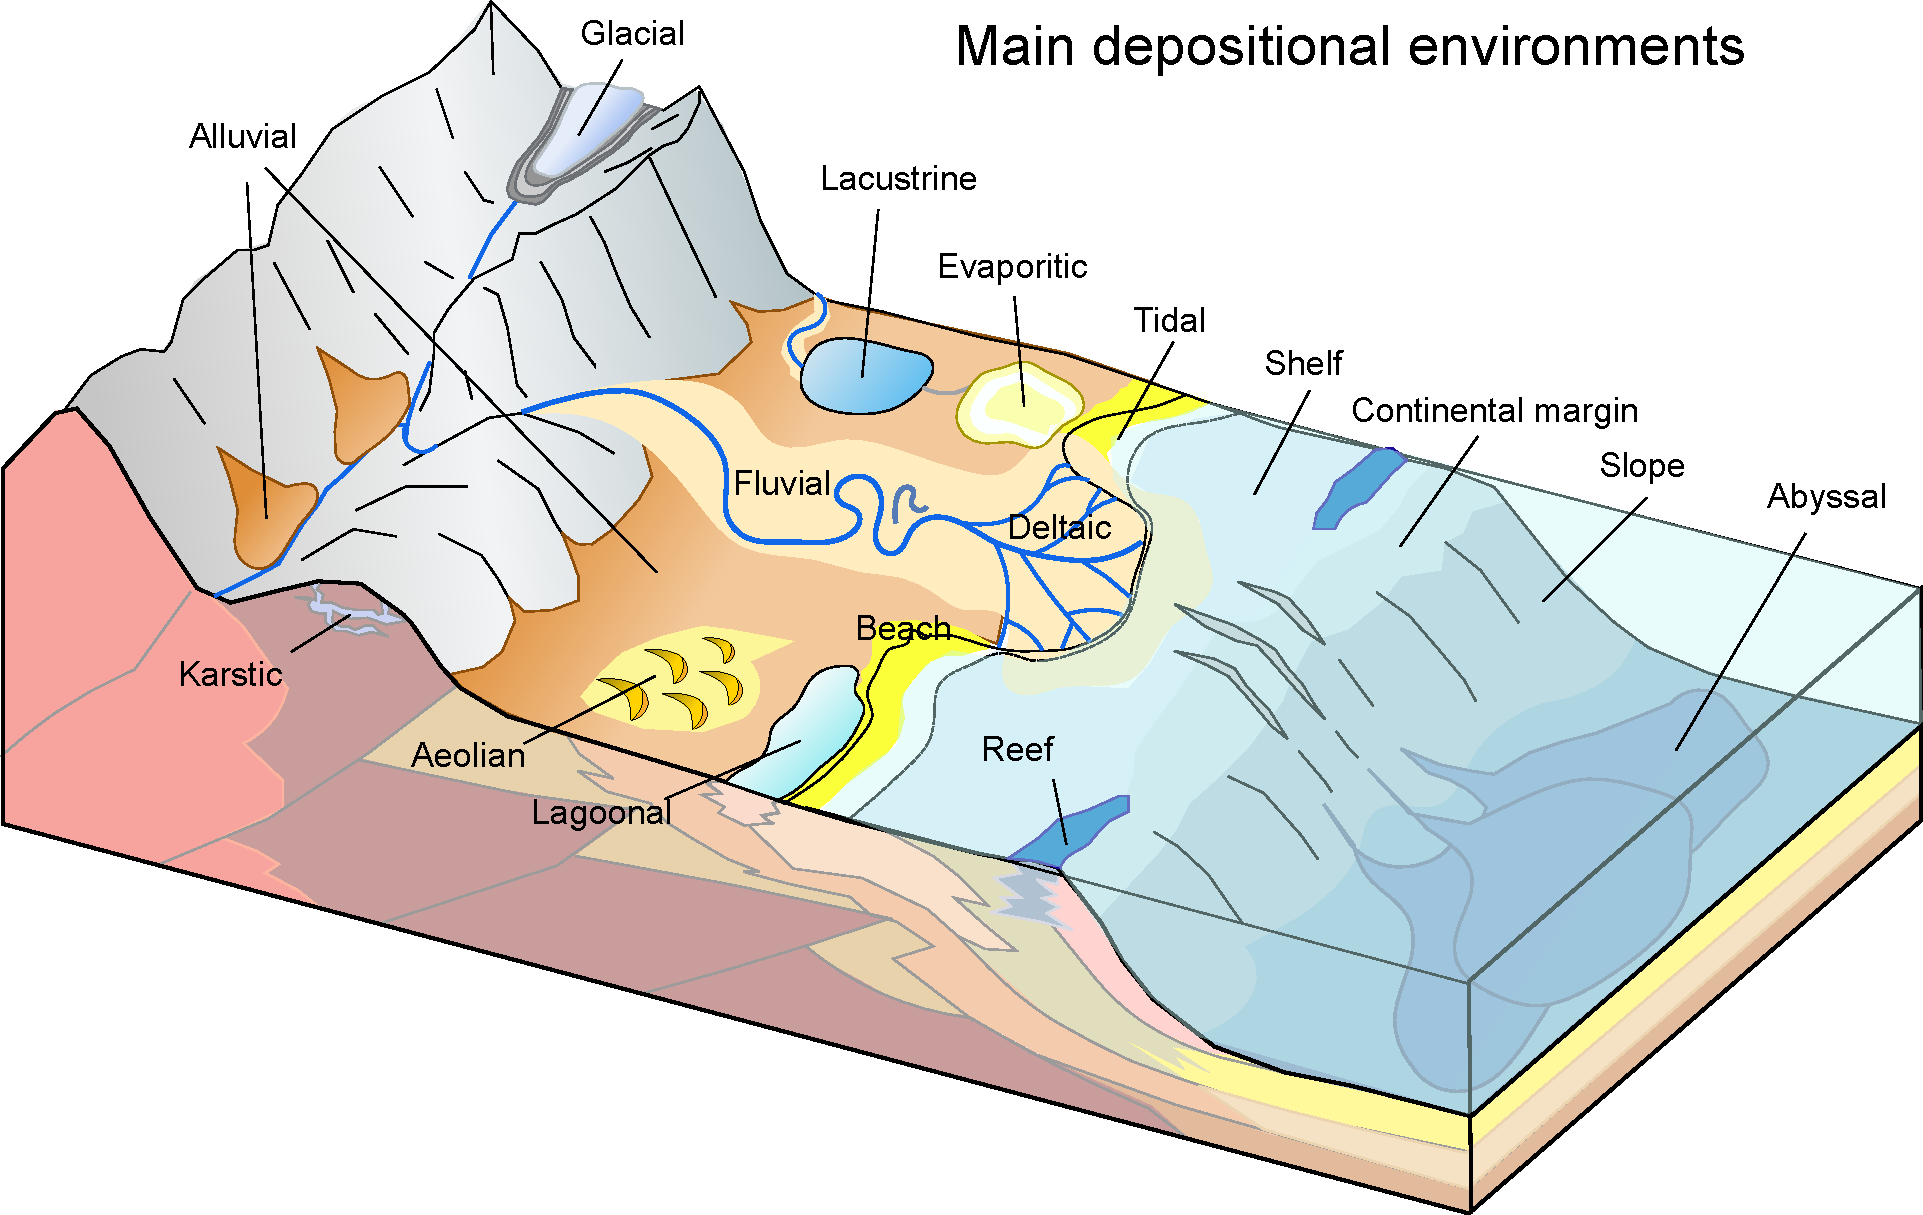
\includegraphics[width=1\twocolwidth]{figures/DepoEnv.pdf}}
  \caption{Schematic diagram of the main depositional environments in sedimentary systems.
    Source: \textcite{Mikenorton2018}
  }\label{fig:DepoEnv}
\end{figure*}

If a figure is being placed at the end of the document rather than near its insertion point define the figure optional position argument using a \texttt{!} or use \verb|\clearpage| directly after the figure environment.

\subsection{Figure design}

Figures must be designed with accessibility in mind.
Do not rely on colour alone, use symbols or patterns to assist with differentiation on graphs and other diagrams.

Preferably use the \href{https://fonts.google.com/noto/specimen/Noto+Sans}{Noto Sans} font family as that is what we use for final production.
However, any standard, sans-serif font (e.g., Arial, Helvetica, Verdana) can be used.
Be consistent and only use one font family.

Use at most three (preferably no more than two) different font sizes for annotations on figures.
The standard font size should be \qty{10}{pt} Noto Sans or equivalent.
Regardless of font choice, the minimum character height must be no less than \qty{4.8}{\milli\metre} at final production size for accessibility purposes.
Aim to use larger font sizes (e.g., \qty{10}{pt} Noto Sans) to improve accessibility.

Colour schemes \textbf{must} be colour-vision deficiency safe (e.g.\href{https://zenodo.org/records/8409685}{Scientific Colour Maps}).

\subsection{Maps}

Map figures must have a scale, grid markers of some form, and state the coordinate reference system of their projection.
\autoref{fig:KatiThanda} is an exemplar of minimum requirements for map figures.

Due to the nature of geology being an international science, some maps may have areas of disputed borders or regions.
In these cases, please use the internationally recognised border or region where possible.

\subsection{Indexing and cross-referencing}

Figures and tables should be numbered in order of appearance and cross-referenced in text.
In \LaTeX, use \verb|\autoref{ref}| to handle this.
For example, these are cross-references to \autoref{fig:DepoEnv} and \autoref{TBL:ftwidths} using \verb|autoref|.

For figures with sub-panels, add uppercase letters for indexing purposes as shown in \autoref{fig:KatiThanda}A and \autoref{fig:KatiThanda}B.
If additional sub-indices are required, use parenthesised lowercase Roman numerals, e.g., A(i).

\subsection{Table formatting}
Complex tables present a significant challenge in \LaTeX\space for our volunteer production team.
Please only use tables where needed, and keep them simple.
Complex tables will incur production delays.

Use a table only if there isn’t a simpler way to present your content, such as a paragraph of text or figure.
Each table must be independently understandable, with a clear title or caption, defined abbreviations, and sufficient explanatory notes where needed.
Tables should be numbered sequentially in the order they are cited in the manuscript.
Design tables for readability and accessibility.
The minimum font size should be Noto Sans 8 pt (or equivalent).
Keep tables simple:
\begin{itemize}
  \item use simple structure, clear column headings, consistent terminology, and SI units;
  \item avoid excessive decimal places, duplicated information, empty cells without explanation, and unnecessary formatting;
  \item do not use colour alone to communicate meaning.
\end{itemize}

Large or highly detailed datasets should be deposited in an appropriate repository and cited in the data availability statement rather than included as oversized manuscript tables.
Datasets provided in a form such as CSV, ODS, XLSX, RData, JLD2, HDF5 etc. are better for study reproducibility.

Tables rules are formatted using \href{http://mirrors.ctan.org/macros/latex/contrib/booktabs/booktabs.pdf}{booktabs}.
This means you can use the \verb|\toprule|, \verb|\midrule|, and \verb|\bottomrule| commands within the \verb|tabular| environment.

The \href{http://mirrors.ctan.org/macros/latex/contrib/nicematrix/nicematrix.pdf}{nicematrix} package is also loaded, providing customisation for blocks and the \verb|X| for the flexible column widths.

\autoref{TBL:ftwidths} is a simple example of a one-column wide table with correct styling and using the \verb|NiceTabular*| environment.

To ensure correct widths of tables, please use the provided custom commands
\begin{itemize}
    \item \verb|\onecolwidth| for single-column width
    \item \verb|\twocolwidth| for two-column width
\end{itemize}
as the size of your \verb|NiceTabular*| or \verb|tabular*| environment.

For tables that will extend beyond a single page, \verb|longtable| is available.
If the \verb|longtable| needs to be two columns wide, or in landscape orientation, please see the \verb|example_longtable.tex| for an example of how to format these.
We have placed the longtable at the end of this build to not clutter the primary information.

To place a table that is only a single column wide (i.e. small tables), use the \verb|table| environment.

Otherwise, use the \verb|table*| environment to place a table that will span both page columns.

\textit{NOTE:} \verb|nicematrix| and \verb|longtable| will not work in the same table.

\section{Mathematics}

In general follow the \href{http://mirrors.ctan.org/info/short-math-guide/short-math-guide.pdf}{Short Math Guide (PDF)}.

Use \verb|\vec{x}| for vectors and \verb|\mathbf{M}| for matrices, e.g.
\begin{verbatim}
  \vec{y} = \mathbf{X}\vec{\beta} + \epsilon
\end{verbatim}
will print:
\begin{equation}
  \vec{y} = \mathbf{X}\vec{\beta} + \epsilon
\end{equation}

In-line equations will look like this: $x^2 + y^2 = z^2$, while basic display equations will look like the following:
\begin{equation}
  \overline{x} = \frac{1}{n}\sum_{i = 1}^{i = n}x_{j} = \frac{x_1 + x_2\ldots + x_n}{n}\label{eq:1}
\end{equation}

Multiline equations will look as follows:
\begin{multline}
  \hat{\rho}_{OP}^2\left(\rho^2\right)=1-\frac{n-3}{n-\left(k+1\right)-1}\cdot\\\left(1-\rho^2\right){{_2}F_1}\left(1,1;\frac{n-\left(k+1\right)-1}{2};1-\rho^2\right) \label{eq:2}
\end{multline}

Finally, aligned equations will look like this:
\begin{align}
  \sum\nolimits\left(x_i-\varepsilon_1\right)\left(x_i-\varepsilon_2\right)\left(x_i-\varepsilon_3\right)\left(x_i-\varepsilon_4\right)=0 \\
  \sum\nolimits{x_i\left(x_i-\varepsilon_1\right)\left(x_i-\varepsilon_2\right)\left(x_i-\varepsilon_3\right)\left(x_i-\varepsilon_4\right)}=0 \\
  \sum\nolimits{{x_i}^2\left(x_i-\varepsilon_1\right)\left(x_i-\varepsilon_2\right)\left(x_i-\varepsilon_3\right)\left(x_i-\varepsilon_4\right)}=0 \\
  \sum\nolimits{{x_i}^3\left(x_i-\varepsilon_1\right)\left(x_i-\varepsilon_2\right)\left(x_i-\varepsilon_3\right)\left(x_i\ -\ \varepsilon_4\right)}=0
\end{align}

\section{Chemical equations}
The \href{https://mirrors.ctan.org/macros/latex/contrib/mhchem/mhchem.pdf}{{mhchem}} package is enabled in the template.
Use \verb|\ce{}| to wrap your chemistry.
For example, \verb|\ce{^{87}_{37}{Rb}+}| prints \ce{^{87}_{37}{Rb}+}.

\section{Referencing}

Appropriate citation of work is mandatory.
While peer-reviewed literature should be the primary sources on which you rely, material considered to be \textit{grey literature} such as pre-prints, theses, government reports, conference papers etc. should be appropriately cited.

The \Sedimentologika\ class uses the \href{https://mirrors.ctan.org/biblio/citation-style-language/citation-style-language-doc.pdf}{citation-style-langauge} package for referencing.

Use \verb|\cite{}| for parenthetical citations, e.g., \cite{ExampleBook}, and \verb|\textcite{}| for in-line text citations, e.g., \textcite{ExampleArticle} stated that this is an awesome template.
Prefixes, suffices, and pointers can be added as optional arguments, e.g.,
\verb|\cite[prefix = {e.g., },|
\verb|suffix={and references therein}]|
\verb|{ExampleThesis}|
will produce \cite[prefix = {e.g., }, suffix={and references therein}]{ExampleThesis}.

The following is to enable generation of a reference list with examples for an article \cite{ExampleArticle}, book \cite{ExampleBook}, book section \cite{ExampleBookSection}, dataset \cite{ExampleDataset}, map \cite{ExampleMap}, preprint \cite{ExamplePreprint}, report \cite{ExampleReport}, software \cite{ExampleSoftware} and thesis \cite{ExampleThesis}.

\section{Conclusions}
This is a mandatory section, replace this text.

Thanks for using the \Sedimentologika\space \LaTeX\space template for preparing your article.

% ---------------------------------------------------------------------------------------- %
%                              Post article matter goes here
% ---------------------------------------------------------------------------------------- %
\acknowledgements{
  Replace this text with your acknowledgements.
}

% This is your data (and code) availability statement - it is mandatory, you must make your
% data and code available via a repository such as Zenodo (Data), GitHub (Code - use Zenodo
% to generate a doi see https://help.zenodo.org/docs/github/) etc.
%
% "Available upon request" is not an allowable statement.
% Please contact Sedimentologika if your data cannot be made available due to legal reasons
%
\datacode{
  Data used in this paper is hosted on Zenodo at \href{https://doi.org/10.1000/182}{doi.org/10.1000/182}, \verb|\cite{ExampleCitation}|.

  The code used in this paper is available via \href{https://example.com} and archived on Zenodo at \href{https://doi.org/10.1000/182}{doi.org/10.1000/182}, \verb|\cite{ExampleCitation}|.
}

\supplementarymaterial{
  If you have any additional supplementary material hosted in a repository for this manuscript please replace this with a statement linking to the doi, and add the citation,
  e.g. Supplementary material for this paper can be found at \href{https://doi.org/10.1000/182}{doi.org/10.1000/182} \verb|\cite{ExampleCitation}|.
}

\conflictofinterest{
  The authors declare they do not have any tangible or perceived conflicts of interest with regard to this research.
}% change as appropriate, this is mandatory

\artificialintelligence{
  All research, analysis, writing, and editing were performed without generative AI assistance.
} % change as appropriate, this is mandatory

\funding{
  Declare sources of funding for this research.
} % change as appropriate, this is mandatory if stating no external funding sources

\printbibliography % uncomment this when you've added you reference library file.

% ---------------------------------------------------------------------------------------- %
%                              Long table example
% ---------------------------------------------------------------------------------------- %
\onecolumn
% SPDX-FileCopyrightText: Copyright © 2026-present Sedimentologika
% SPDX-FileContributor: Jarred C. Lloyd
%
% SPDX-License-Identifier: LPPL-1.3c

\begin{longtable}{p{0.13\textwidth} p{0.12\textwidth} p{0.12\textwidth} p{0.12\textwidth} p{0.12\textwidth} p{0.12\textwidth} p{0.12\textwidth}}
  \caption{Summary of laser conditions and materials analysed in each session.}
  \label{TBL:zircon}\\
  \toprule
  Session Date  & Material  & Spot Diameter (\unit{\micro\metre}) &  Repetition Rate (\unit{\hertz})  & Nominal Fluence (\unit{\joule\per\centi\metre\squared})  & Measured Fluence (\unit{\joule\per\centi\metre\squared})  & Ablation Time (\unit{\second}) \\
  \midrule
  \endfirsthead

  \multicolumn{7}{l}{\textit{table continued from previous page}}\\
  \midrule[0.1pt]
  Session Date  & Material  & Spot Diameter (\unit{\micro\metre}) &  Repetition Rate (\unit{\hertz}) & Nominal Fluence (\unit{\joule\per\centi\metre\squared})  & Measured Fluence (\unit{\joule\per\centi\metre\squared})  & Ablation Time (\unit{\second}) \\
  \midrule
  \endhead

  \multicolumn{7}{r}{\textit{continued on next page\dots}}\\
  \endfoot

  \bottomrule
  \endlastfoot

  2020-02-24 & zircon  & 29 & 5 & 2 &  & 30 \\
  2020-02-24 & glass & 29 & 5 & 3.5 &  & 30 \\
  2020-02-24 & glass & 51 & 5 & 3.5 &  & 30 \\
  2020-02-26 & zircon & 29 & 5 & 2 &  & 30 \\
  2020-02-26 & glass & 29 & 5 & 3.5 &  & 30 \\
  2020-02-26 & glass & 51 & 5 & 3.5 &  & 30 \\
  2020-05-06 & zircon & 19 & 5 & 2 &  & 40 \\
  2020-05-06 & glass & 19 & 5 & 3.5 &  & 40 \\
  2020-05-06 & glass & 51 & 5 & 3.5 &  & 40 \\
  2020-05-08 & glass & 43 & 5 & 3.5 &  & 40 \\
  2020-05-11 & zircon & 29 & 5 & 2 &  & 40 \\
  2020-05-11 & glass & 29 & 5 & 3.5 &  & 40 \\
  2020-05-11 & glass & 51 & 5 & 3.5 &  & 40 \\
  2021-03-30 & zircon & 29 & 5 & 2 &  & 30 \\
  2021-03-30 & glass & 43 & 5 & 3.5 &  & 30 \\
  2021-03-31 & zircon & 30 & 5 & 2 &  & 40 \\
  2021-03-31 & glass & 43 & 5 & 3.5 &  & 40 \\
  2021-05-06 & zircon & 30 & 5 & 2 &  & 40 \\
  2021-05-06 & glass & 43 & 5 & 3.5 &  & 40 \\
  2021-09-06 & zircon & 30 & 5 & 2 &  & 30 \\
  2021-09-06 & glass & 43 & 5 & 3.5 &  & 30 \\
  2021-09-06 & monazite & 20 & 5 & 2 & & 30 \\
  2022-01-19 & baddeleyite & 20 & 5 & 2 & & 30 \\
  2022-01-19 & zircon & 20 & 5 & 2 & & 30 \\
  2022-01-19 & glass & 43 & 5 & 3.5 & & 30 \\
  2022-01-19 & apatite & 30 & 5 & 3.5  &  & 30 \\
  2022-02-01 & monazite & 13 & 5 & 2 & 1.9  & 30 \\
  2022-02-01 & xenotime & 13 & 5 & 2 & 1.9  & 30 \\
  2022-02-01 & glass & 43 & 5 & 3.5 & 3.6  & 30 \\
  2022-04-01 & glass & 43 & 5 & 3.5 & 3.4  & 30 \\
  2022-04-21 & apatite & 30 & 5 & 3.5 & 3.4  & 30 \\
  2022-04-21 & zircon & 30 & 5 & 2 & 2  & 30 \\
  2022-04-21 & glass & 43 & 5 & 3.5 & 3.4  & 30 \\
  2022-05-31 & glass & 43 & 5 & 5 & 5.2  & 30 \\
  2022-05-31 & monazite & 13 & 5 & 2 & 1.9  & 30 \\
  2022-05-31 & xenotime & 13 & 5 & 2 & 1.9  & 30 \\
  2022-06-20 & zircon & 30 & 5 & 2 & 2.1  & 30 \\
  2022-06-20 & glass & 43 & 5 & 3.5 & 3.6  & 30 \\
  2022-06-20 & xenotime & 13 & 5 & 2 & 2.1  & 30 \\
  2022-06-29 & glass & 43 & 5 & 3.5 & 3.4  & 30 \\
  2022-06-29 & xenotime & 13 & 5 & 2 & 1.9  & 30 \\
  2022-07-08 & glass & 43 & 5 & 3.5 & 3.6  & 40 \\
  2022-07-08 & rutile & 43 & 5 & 5 & 5.2  & 40 \\
  2022-08-30 & monazite & 20 & 5 & 2 & 2  & 30 \\
  2022-08-30 & zircon & 20 & 5 & 2 & 2  & 30 \\
  2022-10-10 & glass & 43 & 5 & 3.5 & 3.4  & 30 \\
  2022-10-10 & zircon & 30 & 5 & 2 & 1.9  & 30 \\
  2022-10-11 & glass & 30 & 5 & 3.5&  3.4  & 30 \\
  2022-10-11 & zircon & 43 & 5 & 2 & 1.9  & 30 \\
  2022-12-09 & glass & 43 & 5 & 3.5 & 3.5  & 40 \\
  2022-12-09 & rutile & 43 & 5 & 5 & 4.9  & 40 \\
  2023-02-20 & apatite & 30 & 5 & 3.5 & 3.5  & 30 \\
  2023-02-20 & glass & 30 & 5 & 3.5 & 3.5  & 30 \\
  2023-02-20 & zircon & 30 & 5 & 2 & 1.9  & 30 \\
  2023-03-22 & monazite & 13 & 5 & 2 & 1.8  & 30 \\
  2023-03-22 & xenotime & 13 & 5 & 2 & 1.8  & 30 \\
  2023-04-21 & glass & 43 & 5 & 3.5 & 3.5  & 30 \\
  2023-04-21 & apatite & 43 & 5 & 3.5 & 3.5  & 30 \\
  2023-04-21 & zircon & 30 & 5 & 2 & 2  & 30 \\
  2023-05-09 & glass & 43 & 5 & 3.5 & 3.5  & 40 \\
  2023-05-23 & glass & 43 & 5 & 3.5 & 3.6  & 40 \\
  2023-05-29 & glass & 43 & 5 & 3.5 & 3.4  & 30 \\
  2023-05-29 & monazite & 13 & 5 & 2 & 2.1  & 30 \\
  2023-06-30 & glass & 30 & 5 & 3.5 & 3.4  & 30 \\
  2023-06-30 & apatite & 30 & 5 & 3.5 & 3.4  & 30 \\
  2023-07-11 & glass & 43 & 5 & 3.5 & 3.5  & 40 \\
  2023-07-11 & zircon & 20 & 5 & 2 & 1.9  & 40 \\
  2023-11-24 & apatite & 30 & 5 & 3.5 & 3.5  & 30 \\
  2023-11-24 & baddeleyite & 30 & 5 & 2 & 2  & 30 \\
  2023-11-24 & monazite & 20 & 5 & 2 & 2  & 30 \\
  2023-11-24 & rutile & 43 & 5 & 5 & 4.9  & 30 \\
  2023-11-24 & titanite & 43 & 5 & 5 & 4.9  & 30 \\
  2023-11-24 & xenotime & 20 & 5 & 2 & 2  & 30 \\
  2023-11-24 & zircon & 30 & 5 & 2 & 2  & 30 \\
  2023-11-24 & glass & 30 & 5 & 3.5&  3.5  & 30 \\
  2024-04-29 & apatite & 30 & 5 & 3.5 & 3.5  & 40 \\
  2024-04-29 & baddeleyite & 30 & 5 & 2 & 2.1  & 40 \\
  2024-04-29 & cassiterite & 43 & 5 & 5 & 5.1  & 40 \\
  2024-04-29 & monazite & 20 & 5 & 2 & 2.1  & 40 \\
  2024-04-29 & rutile & 43 & 5 & 5 & 5.1  & 40 \\
  2024-04-29 & titanite & 43 & 5 & 5 & 5.1  & 40 \\
  2024-04-29 & xenotime & 20 & 5 & 2 & 2.1  & 40 \\
  2024-04-29 & zircon & 30 & 5 & 2 & 2.1  & 40 \\
  2024-04-29 & glass & 30 & 5 & 3.5 & 3.5  & 40 \\
\end{longtable} % a way to keep complicated, or long tables from cluttering this main file.
\twocolumn

\end{document}
